\documentclass[aspectratio=169]{ctexbeamer}
% \usetheme{Berkeley}%使用Berkeley主题
\usefonttheme[onlymath]{serif}
\usepackage{amsmath}
\usepackage{tcolorbox}
\usepackage[fontsize=15pt]{fontsize}
\usepackage{fancyhdr}
\usepackage{tikz}
\usepackage{tikz-3dplot}
\usetikzlibrary{decorations.pathreplacing}%使用大括号
\usetikzlibrary{calligraphy} %calligraphy 书法风格
% \usetikzlibrary{positioning}
\usetikzlibrary{calc}
\usetikzlibrary{backgrounds} %特定的绘图操作置于背景层
\usetikzlibrary{3d}

\pagestyle{fancy}
\fancyhf{} % 清除当前头部和脚部的所有内容
\renewcommand{\headrulewidth}{0pt} % 去掉上边线
% \cfoot{\large\thepage} % 将页码置于中央位置

\usepackage{xeCJK} % 用于处理中文排版
\setCJKmainfont[AutoFakeBold=true]{STKaiti} % 设置中文主字体为华文楷体 %AutoFakeBold 添加加粗的效果(自动伪粗体),能使用 \textbf了
\usepackage{fontspec}
% 设置英文主字体为 Times New Roman
\setmainfont{Times New Roman}
\usepackage{graphicx}
\begin{document}

\title{高一下立体几何复习}
\date{2025 年 5 月 15 日}
\begin{frame}{}{}%大标题和小标题的设置与否根据自身需求设定
    \titlepage{}
\end{frame}
\begin{frame}{}{}
    % \usetikzlibrary{decorations.pathreplacing}%使用大括号
% \usetikzlibrary{calligraphy} %calligraphy 书法风格
% % \usetikzlibrary{positioning}
% \usetikzlibrary{calc}
% \usetikzlibrary{backgrounds} %特定的绘图操作置于背景层
% \usetikzlibrary{3d}

% 将代码中的顶点名称 A、B、C、D 替换为 D、C、B、A
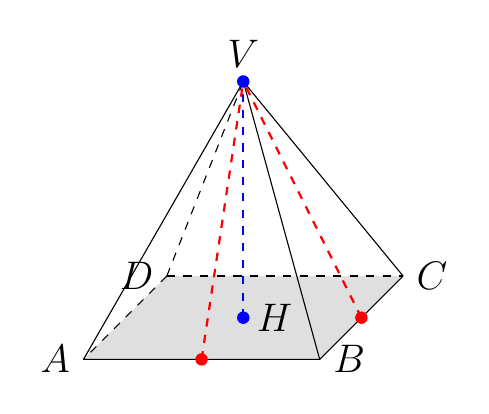
\begin{tikzpicture}[scale=3,
    y={(-0.353cm,-0.353cm)}, % 设置 x 轴方向
    x={(1cm,0cm)},            % 设置 y 轴方向
    z={(0cm,1cm)}             % 设置 z 轴方向
]%斜二测画法
\coordinate (D) at (0,0,0);
\coordinate (C) at (1,0,0);
\coordinate (B) at (1,1,0);
\coordinate (A) at (0,1,0);
\coordinate (V) at (0.5,0.5,1);

\coordinate (H) at (0.5,0.5,0);
% 计算中点
\coordinate (H') at ($(A)!0.5!(B)$);
\coordinate (H'') at ($(C)!0.5!(B)$);
%填充底面
\fill[lightgray,opacity=0.5] (D) -- (C) -- (B) -- (A) -- cycle;

% 绘制底面
\draw (C) -- (B) -- (A);

% 绘制侧面
\draw[dashed] (D) -- (V);
\draw[dashed] (D) -- (A);
\draw[dashed] (D) -- (C);
\draw (C) -- (V);
\draw (B) -- (V);
\draw (A) -- (V);


\draw[thick,blue,dashed] (H) -- (V); %棱柱的高

\draw[thick,red,dashed] (H') -- (V); %棱柱的斜高
\draw[thick,red,dashed] (H'') -- (V); %棱柱的斜高

% 标记顶点
\node[ left] at (D) {$D$};
\node[ right] at (C) {$C$};
\node[ right] at (B) {$B$};
\node[left] at (A) {$A$};
\node[above] at (V) {$V$};
\node[right] at (H) {$H$};

%绘制圆点
\fill[blue] (V) circle (0.75pt);
\fill[blue] (H) circle (0.75pt);
\fill[red] (H') circle (0.75pt);
\fill[red] (H'') circle (0.75pt);
% \node[circle, fill=blue, inner sep=1.5pt] at (V) {};
% \node[circle, fill=blue, inner sep=1.5pt] at (H) {};
\end{tikzpicture}

\end{frame}





\end{document}